\documentclass{article}
\usepackage{mathtools,amssymb}
\usepackage{float,graphicx}
\usepackage{nopageno}
\usepackage[letterpaper]{geometry}

\setlength{\parindent}{0in}


\begin{document}

\section*{Combinations}

\textbf{Definition:} For non-negative integers $n$ and $k$ with $0\leq k\leq n$,
\begin{equation*}
\binom{n}{k} = C(n,k) = {}_nC_k = \frac{n(n - 1)(n - 2)\cdots (n - k + 1)}{k!} = \frac{n!}{k!(n - k)!}
\end{equation*}
is the number of ways to select, from $n$ distinct objects, an (unordered) collection of $k$ of them.
\begin{enumerate}
\item \begin{enumerate}
\item How many distinct line segments can be drawn that connect two vertices of a regular octagon? Include the sides of the octagon in your count.\vspace{1cm}
\item A \emph{diagonal} of a convex polygon is a segment connecting two non-adjacent vertices of the polygon. How many diagonals does a regular octagon have?
\end{enumerate}\vspace{1cm}
\item Maraya is going to buy six cookies at the bakery. She will choose from sugar, ginger, chocolate, and peanut butter cookies. How many different assortments of cookies can she buy if she will buy at least one of each of the four kinds of cookies?\vspace{1cm}
\item An ant needs to crawl from $A$ to $B$ along the gridlines in a path that is as short as possible. How many such paths are available?
\begin{figure}[H]
\centering
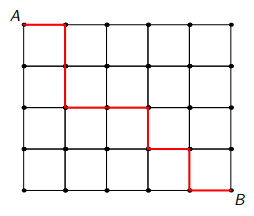
\includegraphics[scale=0.5]{grid.png}
\end{figure}
\item There are 7 dots on a circle and each pair of distinct dots is joined by a line segment.
\begin{enumerate}
\item How many line segments are there connecting any 2 of these 7 dots?\vspace{1cm}
\item ($\star$) What is the maximum possible number of intersection points inside the circle that can be formed by these line segments?\vspace{1cm}
\item ($\star$) What is the maximum possible number of regions inside the circle that can be formed by these line segments?
\end{enumerate}
\end{enumerate} 


% \newpage

% \section*{Repeated Elements}

% \begin{enumerate}
% \item If all the letters of the word $SYZYGY$\footnote{``In astronomy, a roughly straight-line configuration of three or more celestial bodies.''} are used, in how many different ways can the six letters be arranged in a six-letter string?\vspace{4cm}
% \item In how many different ways can the letters in the word $PEOPLE$ be scrambled, including the original spelling $PEOPLE$?\vspace{4cm}
% \item (2006 State Sprint Problem 28) Derek's phone number, 336-7624, has the property that the three-digit prefix, 336, equals the product of the last four digits, $7\times 6\times 2\times 4$. How many seven-digit phone numbers beginning with 336 have this property?
% \end{enumerate}


\newpage

\section*{Extensions}
\vspace{1cm}
\begin{enumerate}
\item \underline{\hspace{3in}}\vspace{1cm}
\item \underline{\hspace{3in}} (2012 School Team)\vspace{1cm}
\item \underline{\hspace{3in}} (2012 National Sprint Problem 25)\vspace{1cm}
\item \underline{\hspace{3in}}\vspace{1cm}
\item \underline{\hspace{3in}} (2010 Chapter Team)\vspace{1cm}
\item \underline{\hspace{3in}} (2012 State Sprint Problem 27)\vspace{1cm}
\item \underline{\hspace{3in}}\vspace{1cm}
\item \underline{\hspace{3in}}
\end{enumerate}


\newpage

\section*{Extra Problems}

\begin{enumerate}
\item Solve the following system of equations:
\begin{align*}
a + b + c + d + e + f &= 4, \\
32a + 16b + 8c + 4d + 2e + f &= 8, \\
243a + 81b + 27c + 9d + 3e + f &= 14, \\
1024a + 256b + 64c + 16d + 4e + f &= 22, \\
3125a + 625b + 125c + 25d + 5e + f &= 32, \\
7776a + 1296b + 216c + 36d + 6e + f &= 44.
\end{align*}
Express your answer as an ordered 6-tuple $(a,b,c,d,e,f)$.\vspace{3cm}
\item ($\star$) For how many ordered pairs of non-negative integers $(n,k)$ does $\dbinom{n}{k} = 3003$?\vspace{3cm}
\item A pyramid has a square base $ABCD$ of side length 1 and an apex $P$ located directly above point $A$ (relative to the plane of $ABCD$) with $AP = 1$. Find the total surface area of the pyramid, expressing your answer in simplest radical form.\vspace{3cm}
\item Let $A$ be the number of perfect square divisors of $20!$ and let $B$ be the number of perfect square divisors of $25!$. Compute $B - A$.
\end{enumerate}


\end{document}